\documentclass[12pt,a4paper]{article}
\usepackage[utf8]{inputenc}
\usepackage[T1]{fontenc}
\usepackage[margin=2.5cm]{geometry}
\usepackage{graphicx}
\usepackage{hyperref}
\usepackage{enumitem}
\usepackage{xcolor}
\usepackage{tikz}
\usetikzlibrary{shapes.geometric, arrows, positioning, fit}
\usepackage{fancyhdr}
\usepackage{titlesec}
\usepackage{listings}

\definecolor{primary}{RGB}{220, 38, 38}
\definecolor{codebg}{RGB}{248, 249, 250}

\lstset{
    backgroundcolor=\color{codebg},
    basicstyle=\ttfamily\small,
    breaklines=true,
    frame=single
}

\hypersetup{
    colorlinks=true,
    linkcolor=primary,
    urlcolor=primary
}

\pagestyle{fancy}
\fancyhf{}
\fancyhead[L]{Software Development Project}
\fancyhead[R]{Lecture 8: System Design}
\fancyfoot[C]{\thepage}

\title{\textbf{Lecture 8: System Design and Architecture}\\[0.5cm]\large Building the Blueprint for Your Software}
\author{State University of Zanzibar (SUZA)\\BSc Computer Science}
\date{}

\begin{document}

\maketitle
\tableofcontents
\newpage

\section{Introduction to System Design}

\subsection{What is System Design?}
System design is the process of defining the architecture, components, modules, interfaces, and data flow of a system to satisfy specified requirements.

\subsection{Why Design Matters}
\begin{itemize}
    \item Provides a roadmap for development
    \item Identifies potential problems early
    \item Enables parallel development by teams
    \item Facilitates maintenance and scalability
    \item Ensures all team members have shared understanding
\end{itemize}

\section{Architecture Patterns}

\subsection{Monolithic Architecture}

\begin{center}
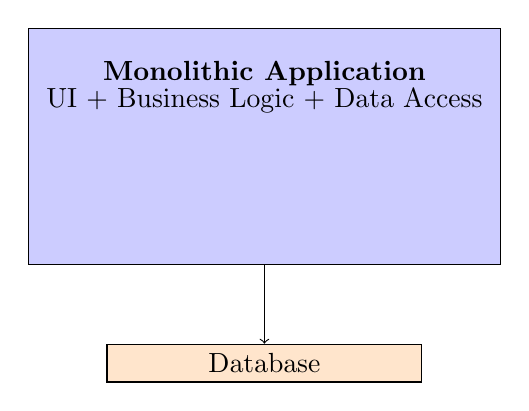
\begin{tikzpicture}
    \node[draw, rectangle, minimum width=6cm, minimum height=3cm, fill=blue!20] (mono) {};
    \node at (mono.north) [below=0.3cm] {\textbf{Monolithic Application}};
    \node at (mono.center) [above=0.3cm] {UI + Business Logic + Data Access};
    \node[draw, rectangle, minimum width=4cm, fill=orange!20, below=1cm of mono] (db) {Database};
    \draw[->] (mono) -- (db);
\end{tikzpicture}
\end{center}

\textbf{Characteristics:}
\begin{itemize}
    \item Single deployable unit
    \item All components tightly coupled
    \item Simple to develop and deploy initially
\end{itemize}

\textbf{Best For:} Small projects, student projects, MVPs

\textbf{Drawbacks:} Hard to scale, difficult to maintain as it grows

\subsection{Layered (N-Tier) Architecture}

\begin{center}
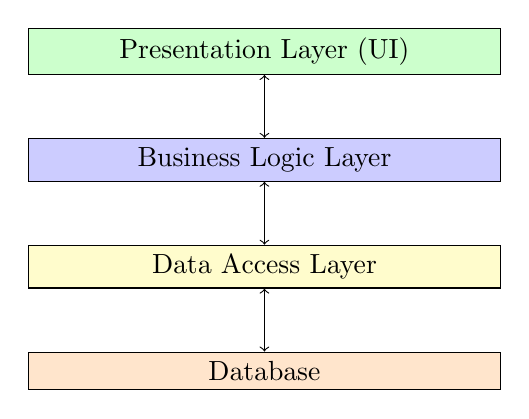
\begin{tikzpicture}[node distance=0.8cm]
    \node[draw, rectangle, minimum width=6cm, fill=green!20] (pres) {Presentation Layer (UI)};
    \node[draw, rectangle, minimum width=6cm, fill=blue!20, below=of pres] (bus) {Business Logic Layer};
    \node[draw, rectangle, minimum width=6cm, fill=yellow!20, below=of bus] (data) {Data Access Layer};
    \node[draw, rectangle, minimum width=6cm, fill=orange!20, below=of data] (db) {Database};

    \draw[<->] (pres) -- (bus);
    \draw[<->] (bus) -- (data);
    \draw[<->] (data) -- (db);
\end{tikzpicture}
\end{center}

\textbf{Layers:}
\begin{enumerate}
    \item \textbf{Presentation Layer:} User interface (HTML, React, etc.)
    \item \textbf{Business Logic Layer:} Application rules and processing
    \item \textbf{Data Access Layer:} Database operations
    \item \textbf{Database Layer:} Data storage
\end{enumerate}

\textbf{Best For:} Most web applications, enterprise software

\subsection{MVC (Model-View-Controller)}

\begin{center}
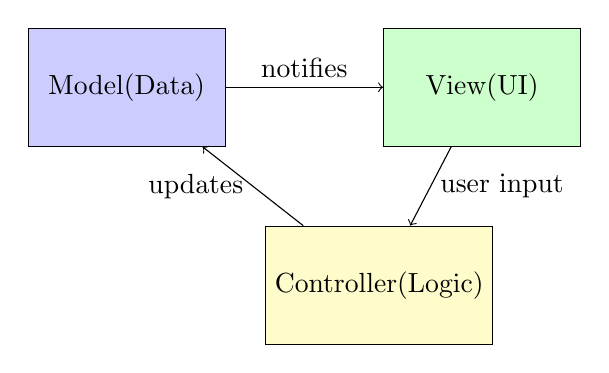
\begin{tikzpicture}[node distance=2cm]
    \node[draw, rectangle, minimum width=2.5cm, minimum height=1.5cm, fill=blue!20] (model) {Model\\(Data)};
    \node[draw, rectangle, minimum width=2.5cm, minimum height=1.5cm, fill=green!20, right=of model] (view) {View\\(UI)};
    \node[draw, rectangle, minimum width=2.5cm, minimum height=1.5cm, fill=yellow!20, below right=1cm and 0.5cm of model] (controller) {Controller\\(Logic)};

    \draw[->] (controller) -- node[left] {updates} (model);
    \draw[->] (model) -- node[above] {notifies} (view);
    \draw[->] (view) -- node[right] {user input} (controller);
\end{tikzpicture}
\end{center}

\textbf{Components:}
\begin{itemize}
    \item \textbf{Model:} Data and business logic
    \item \textbf{View:} User interface display
    \item \textbf{Controller:} Handles user input, updates model
\end{itemize}

\textbf{Popular Frameworks:} Django (Python), Laravel (PHP), Ruby on Rails

\subsection{Client-Server Architecture}

\begin{center}
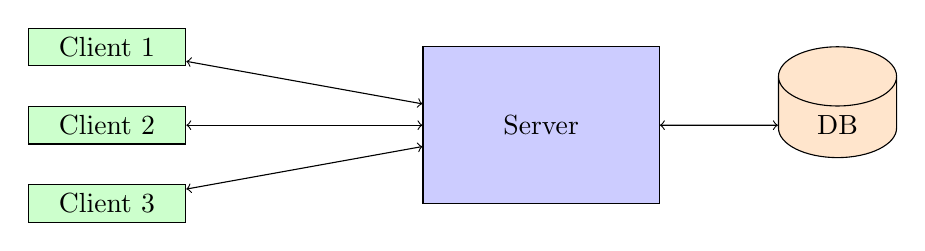
\begin{tikzpicture}[node distance=3cm]
    \node[draw, rectangle, minimum width=2cm, fill=green!20] (c1) {Client 1};
    \node[draw, rectangle, minimum width=2cm, fill=green!20, below=0.5cm of c1] (c2) {Client 2};
    \node[draw, rectangle, minimum width=2cm, fill=green!20, below=0.5cm of c2] (c3) {Client 3};

    \node[draw, rectangle, minimum width=3cm, minimum height=2cm, fill=blue!20, right=of c2] (server) {Server};
    \node[draw, cylinder, shape border rotate=90, minimum width=1.5cm, fill=orange!20, right=1.5cm of server] (db) {DB};

    \draw[<->] (c1) -- (server);
    \draw[<->] (c2) -- (server);
    \draw[<->] (c3) -- (server);
    \draw[<->] (server) -- (db);
\end{tikzpicture}
\end{center}

\textbf{Best For:} Web applications, mobile apps with backend

\section{Technology Stack Selection}

\subsection{Frontend Technologies}

\begin{tabular}{|l|l|l|}
\hline
\textbf{Technology} & \textbf{Type} & \textbf{Best For} \\
\hline
HTML/CSS/JS & Basics & Simple websites \\
\hline
React & Library & Dynamic SPAs \\
\hline
Vue.js & Framework & Progressive apps \\
\hline
Angular & Framework & Enterprise apps \\
\hline
Bootstrap & CSS Framework & Responsive design \\
\hline
Tailwind CSS & CSS Framework & Custom designs \\
\hline
\end{tabular}

\subsection{Backend Technologies}

\begin{tabular}{|l|l|l|}
\hline
\textbf{Technology} & \textbf{Language} & \textbf{Best For} \\
\hline
Node.js/Express & JavaScript & APIs, real-time apps \\
\hline
Django & Python & Rapid development \\
\hline
Flask & Python & Lightweight APIs \\
\hline
Spring Boot & Java & Enterprise apps \\
\hline
Laravel & PHP & Web applications \\
\hline
Ruby on Rails & Ruby & Startups, MVPs \\
\hline
\end{tabular}

\subsection{Database Selection}

\textbf{Relational Databases (SQL):}
\begin{itemize}
    \item PostgreSQL - Feature-rich, open source
    \item MySQL - Popular, easy to use
    \item SQLite - Lightweight, file-based
\end{itemize}

\textbf{NoSQL Databases:}
\begin{itemize}
    \item MongoDB - Document-based, flexible schema
    \item Redis - In-memory, caching
    \item Firebase - Real-time, mobile apps
\end{itemize}

\textbf{When to Use What:}
\begin{itemize}
    \item \textbf{SQL:} Structured data, complex queries, transactions
    \item \textbf{NoSQL:} Flexible schema, scalability, unstructured data
\end{itemize}

\section{Database Design}

\subsection{Entity-Relationship Diagram (ERD)}

An ERD shows entities (tables) and their relationships.

\textbf{Components:}
\begin{itemize}
    \item \textbf{Entity:} A table (e.g., User, Product, Order)
    \item \textbf{Attribute:} Column in a table (e.g., name, email)
    \item \textbf{Relationship:} Connection between tables
\end{itemize}

\subsection{Relationship Types}

\begin{itemize}
    \item \textbf{One-to-One (1:1):} User has one Profile
    \item \textbf{One-to-Many (1:N):} User has many Orders
    \item \textbf{Many-to-Many (M:N):} Students enroll in Courses
\end{itemize}

\subsection{Example: E-commerce Database}

\begin{lstlisting}
Table: users
- id (PK)
- username
- email
- password_hash
- created_at

Table: products
- id (PK)
- name
- description
- price
- stock_quantity

Table: orders
- id (PK)
- user_id (FK -> users)
- total_amount
- status
- created_at

Table: order_items
- id (PK)
- order_id (FK -> orders)
- product_id (FK -> products)
- quantity
- price
\end{lstlisting}

\subsection{Normalization}

\textbf{Purpose:} Reduce data redundancy and improve data integrity.

\textbf{Normal Forms:}
\begin{enumerate}
    \item \textbf{1NF:} No repeating groups, atomic values
    \item \textbf{2NF:} 1NF + no partial dependencies
    \item \textbf{3NF:} 2NF + no transitive dependencies
\end{enumerate}

\section{API Design}

\subsection{What is an API?}
Application Programming Interface - a way for software components to communicate.

\subsection{REST API Principles}

\begin{itemize}
    \item \textbf{Stateless:} Each request contains all needed information
    \item \textbf{Resource-based:} URLs represent resources
    \item \textbf{HTTP Methods:} Use appropriate methods for actions
    \item \textbf{JSON:} Standard data format
\end{itemize}

\subsection{HTTP Methods}

\begin{tabular}{|l|l|l|}
\hline
\textbf{Method} & \textbf{Action} & \textbf{Example} \\
\hline
GET & Read/Retrieve & GET /users \\
\hline
POST & Create & POST /users \\
\hline
PUT & Update (full) & PUT /users/1 \\
\hline
PATCH & Update (partial) & PATCH /users/1 \\
\hline
DELETE & Delete & DELETE /users/1 \\
\hline
\end{tabular}

\subsection{RESTful URL Design}

\begin{lstlisting}
Good URLs:
GET    /users           - List all users
GET    /users/1         - Get user with id 1
POST   /users           - Create new user
PUT    /users/1         - Update user 1
DELETE /users/1         - Delete user 1
GET    /users/1/orders  - Get orders for user 1

Bad URLs:
GET /getUsers
GET /getUserById?id=1
POST /createNewUser
GET /deleteUser/1
\end{lstlisting}

\subsection{API Response Format}

\begin{lstlisting}
Success Response:
{
    "success": true,
    "data": {
        "id": 1,
        "name": "John Doe",
        "email": "john@example.com"
    }
}

Error Response:
{
    "success": false,
    "error": {
        "code": 404,
        "message": "User not found"
    }
}
\end{lstlisting}

\subsection{HTTP Status Codes}

\begin{tabular}{|l|l|}
\hline
\textbf{Code} & \textbf{Meaning} \\
\hline
200 OK & Success \\
\hline
201 Created & Resource created \\
\hline
400 Bad Request & Invalid input \\
\hline
401 Unauthorized & Authentication required \\
\hline
403 Forbidden & Not allowed \\
\hline
404 Not Found & Resource doesn't exist \\
\hline
500 Server Error & Internal error \\
\hline
\end{tabular}

\section{User Interface Design}

\subsection{UI/UX Principles}

\begin{itemize}
    \item \textbf{Consistency:} Similar elements behave similarly
    \item \textbf{Feedback:} Show users what's happening
    \item \textbf{Simplicity:} Don't overwhelm users
    \item \textbf{Accessibility:} Design for all users
    \item \textbf{Mobile-first:} Design for small screens first
\end{itemize}

\subsection{Wireframes vs Mockups}

\begin{itemize}
    \item \textbf{Wireframe:} Low-fidelity, shows layout and structure
    \item \textbf{Mockup:} High-fidelity, shows visual design
    \item \textbf{Prototype:} Interactive, shows user flow
\end{itemize}

\subsection{Tools for UI Design}

\begin{itemize}
    \item Figma (recommended, free)
    \item Adobe XD
    \item Sketch
    \item Balsamiq (wireframes)
    \item Paper and pencil!
\end{itemize}

\section{Security Design}

\subsection{Authentication vs Authorization}

\begin{itemize}
    \item \textbf{Authentication:} Who are you? (Login)
    \item \textbf{Authorization:} What can you do? (Permissions)
\end{itemize}

\subsection{Authentication Methods}

\begin{itemize}
    \item \textbf{Session-based:} Server stores session data
    \item \textbf{Token-based (JWT):} Client stores token
    \item \textbf{OAuth:} Third-party authentication (Google, GitHub)
\end{itemize}

\subsection{Security Best Practices}

\begin{enumerate}
    \item Hash passwords (use bcrypt)
    \item Use HTTPS everywhere
    \item Validate all user input
    \item Prevent SQL injection (use parameterized queries)
    \item Prevent XSS (escape output)
    \item Implement rate limiting
    \item Keep dependencies updated
\end{enumerate}

\section{Design Document Template}

Your System Design Document should include:

\begin{enumerate}
    \item \textbf{Introduction:} Purpose and scope
    \item \textbf{Architecture Overview:} High-level diagram
    \item \textbf{Technology Stack:} Frontend, backend, database
    \item \textbf{Database Design:} ERD and schema
    \item \textbf{API Design:} Endpoints and examples
    \item \textbf{UI Design:} Wireframes/mockups
    \item \textbf{Security:} Authentication and authorization
    \item \textbf{Deployment:} How it will be hosted
\end{enumerate}

\section{Summary}

\begin{itemize}
    \item Choose architecture pattern based on project needs
    \item Select appropriate technology stack
    \item Design database with proper normalization
    \item Follow REST principles for APIs
    \item Consider security from the start
    \item Document your design decisions
\end{itemize}

\end{document}
